% This is samplepaper.tex, a sample chapter demonstrating the
% LLNCS macro package for Springer Computer Science proceedings;
% Version 2.20 of 2017/10/04
%
\documentclass[11pt]{llncs}

%
\usepackage[bindingoffset=0mm,margin=2.5cm]{geometry}
\usepackage{graphicx}
\usepackage{float}
\usepackage[ ]{algorithm2e}
\usepackage[ ]{algorithmicx}
\usepackage{newtxmath}
\usepackage{fixltx2e}
\usepackage[printonlyused,withpage]{acronym}
\usepackage{hyperref}

\RestyleAlgo{boxruled}

\def\SPSB#1#2{\rlap{\textsuperscript{#1}}\textsubscript{#2}}

%
% Used for displaying a sample figure. If possible, figure files should
% be included in EPS format.
%
% If you use the hyperref package, please uncomment the following line
% to display URLs in blue roman font according to Springer's eBook style:
% \renewcommand\UrlFont{\color{blue}\rmfamily}

\begin{document}
%
\title{Comparing Different Approaches for Symbolic Execution\\ ECE 653 - Project Report}
%\thanks{Supported by University of Waterloo}}
%
%\titlerunning{Abbreviated paper title}
% If the paper title is too long for the running head, you can set
% an abbreviated paper title here
%
\author{Uditya Laad (20986041) (\email{ulaad@uwaterloo.ca})
\\Karanjot Singh (20928604) (\email{karanjot@uwaterloo.ca})}
% Third Author\inst{3}\orcidID{2222--3333-4444-5555}}
%
\authorrunning{Authors: Uditya Laad, Karanjot Singh}
% First names are abbreviated in the running head.
% If there are more than two authors, 'et al.' is used.
%
\institute{University of Waterloo, Waterloo, ON, N2L 3G1, CA\\
%\url{url}
}

%
\maketitle              % typeset the header of the contribution
%

\vspace{-6mm}


\begin{abstract}
	Symbolic execution has come a long way since its very introduction. Today, we have many sub-categories of symbolic execution techniques aimed at overcoming the challenges and difficulties associated with Static Symbolic Execution (SSE). In this report, we discuss these challenges and how 4 types of symbolic execution techniques, namely – Static Symbolic Execution (SSE), Selective Symbolic Execution (SeSE), Dynamic Symbolic Execution (DSE) (Breadth-first style, Depth-first style), and Symbolic Backward Execution (SBE) compare against each other. To complement this discussion, we have implemented 3 small execution engines, with WLANG as the artifact, using the same structure we had used for creating a Static Symbolic Execution Engine in one of the assignments. We analyze how the 3 new implementations fare against each other for some sample test cases. In the process, we also discuss the design principles, examples and applications of each of these techniques.

	\keywords{Symbolic Execution  \and Static Symbolic Execution \and  Dynamic Symbolic Execution  \and  Selective Symbolic Execution  \and  Symbolic Backward Execution }
\end{abstract}

\vspace{-17mm}
	
$\>$ $\>$ $\>$ 
	\begin{table}[!]	
		\centering
		\setlength{\tabcolsep}{6pt}
		\begin{tabular}{l l l}
			\textbf{Abbreviations:} & SE & Symbolic Execution\\
			& SSE & Static Symbolic Execution\\
			& DSE & Dynamic Symbolic Execution\\
			& SeSE & Selective Symbolic Execution\\
			& SBE & Symbolic Backward Execution\\
			& SAT & Satisfiable\\
			& UNSAT & Unsatisfiable\\
			& AST & Abstract Syntax Tree

		\end{tabular}
	\end{table}

%	\begin{acronym}
%		\acro {n} {Number of Vertices}
%		\acro {k} {Size of Proposed Vertex Cover}
%		\acro {Std. Dev.} {Standard Deviation}
%	\end{acronym}



\section{Introduction} \label{Introduction}
	Symbolic execution (SE) is one of the most widely used techniques to aid software testing. It helps generate test cases for feasible paths in the program, so that useful program paths can be tested instead of just random testing.\cite{4_TP_SE} Symbolic execution traverses the program in consideration, in terms of symbolic expressions, so that multiple feasible paths can be found and respective test cases or satisfying assignments generated.

	\vspace{2mm}

	\textbf{Why Symbolic Execution?} Symbolic execution was introduced in the mid 70’s\cite{2_Survey_SE} to combat the challenges associated with finding good and meaningful test cases for programs under test. Even though we have other techniques such as random testing, fuzzing, etc; majority of those techniques tend to under-approximate the feasible program properties \cite{2_Survey_SE}. Also, some of those techniques, tend to find cases which are either infeasible or take the same execution path as the other test cases (i.e., path duplication). We further discuss how symbolic execution helps overcome these problems so that each new test case is guaranteed to cover a unique path.

	\vspace{2mm}

	\textbf{Key Idea} The main characteristic of symbolic execution is that it maintains the explored path in terms of symbolic expressions, such that all feasible combinations of non-concretized variables can be taken into consideration when deciding whether a particular path can be taken, instead of deciding on the basis of random concrete value for the variables, as is the case with most other random testing techniques. A state in symbolic execution is maintained as a tuple – \cite{2_Survey_SE}

	\vspace{-1mm}

	\begin{equation}
		\begin{split}
			either	\hspace{40mm} \textbf{$ < $ path-condition, symbolic-environment $ > $} \\
			or 	\hspace{2mm} \textbf{$ < $ path-condition, symbolic-environment, concrete-environment $ > $}
		\end{split}
	\end{equation}
	
	where ‘path-condition’ is a first-order Boolean formula that checks for path satisfiability and is updated each time a branch-split (if-then-else, while-do, case, etc), assertion or assumption is encountered. ‘Symbolic-memory-mapping or environment’ maps each defined variable to its symbolic counterpart. Similarly, ‘Concrete-memory-mapping or environment’ maps each defined variable to a concrete assignment, such that the assignments satisfy the path-condition for that state.

	\vspace{2mm}

	Checking path satisfiability and finding the corresponding model (i.e., the satisfying assignment) is mostly done using a ‘Satisfiability-Modulo-Theory (SMT)’ solver. One of the most popular ones in use today in markets is z3-solver by Microsoft \cite{6_MS_Z3}

	\vspace{2mm}

	\textbf{First-hand results} Overall, performing symbolic execution on a program, results in an acyclic directed control flow graph, such that each of the leaf nodes have a satisfiable path condition - with a model, to be used as one of the test cases. \cite{4_TP_SE}

	\vspace{2mm}

We further discuss the many design principles, associated challenges, search strategies and types of symbolic execution engines in detail. Additionally, small implementations of the 3 symbolic execution engines can be found in the project directory, the results of which have been discussed towards the end of this report.




\section{How Symbolic Execution finds bugs?}
	As discussed in the introduction, Symbolic Execution traverses feasible paths and generates respective satisfying assignments which can be utilized as test cases. When the test suite containing these cases is run, the bugs that exist in the respective path are triggered and hence get recorded in the test results. \cite{7_UW_SE} These are the bugs that are found as a result of testing performed, after symbolic execution.

	However, certain bugs can be directly found while we are performing symbolic execution. This requires some extra effort. Some oracles such as assertions are compiled into conditionals such that if the path condition and assertions are together VALID, then there are no bugs. Otherwise, even if there is one case, where the combined boolean formula may not hold; then it can be treated as a potential bug in the program. \cite{7_UW_SE}
	
	\begin{equation}
		\begin{split}
			In \, general, \, \textbf{‘assert (condition)’}  \, can \, be \, expressed \, as \, \\
			 \textbf{‘if not(condition) then raiseError else proceed’} 
		\end{split}
	\end{equation}
	
	
	The assertions can be used for a safety property such as divide by zero, array index out of bounds, nullPointers, etc.; where the implementation can be explicit (provide assertions or checks before the safe operation) or implicit (added at run-time by the symbolic execution engine – which requires the engine to be created/implemented with that aspect in mind.) \cite{7_UW_SE}. Note that, not all execution engines may support the implicit implementation.



\section{Common Properties of Symbolic Execution Techniques }
	Any version of Symbolic execution tends to share the following common properties \cite{2_Survey_SE}:
	\begin{enumerate}
		\item \textbf{Progress:} For every CPU resource and second of time that is consumed by the Symbolic Execution Engine, it is justified by progress in terms of – new paths, update to memory stores, removal of infeasible paths or reporting assertion failure. \cite{2_Survey_SE}

		\vspace{2mm}

		\item \textbf{Uniqueness:} Every new path that is explored should be different from the rest of the paths that have been explored to that point.

		\vspace{2mm}

		\item \textbf{Symbolic update:}  Symbolic expressions are updated (if applicable) at each step of the program that changes the state; irrespective of whether that part of the program is explored concretely or symbolically.

		\vspace{2mm}

		\item \textbf{Maintain History in Path Condition:} ‘Path condition’ at each new step in the execution, must contain all the constraints that had been explored to reach that node.
	\end{enumerate}



\section{Common Challenges with Symbolic Execution}
	Symbolic execution is a very exhaustive process; and even though it produces very good results for the sample programs that we discuss in this report, the same may not hold for programs of bigger size. Following are some of the common challenges faced with all types of symbolic execution techniques, when used with industry and other real-world applications:

    \vspace{-1mm}
    
	\subsubsection{Memory Aliasing}

		Having multiple reference variables pointing to the same address in memory, is something that can be very difficult for an SMT solver to manage. However, SE uses symbolic expressions for the variables and mostly does not take dynamic memory allocation into account. \cite{5_Wiki_SE}

	\vspace{-3mm}

	\subsubsection{Collections}

		Real-world applications tend to use a lot of collections such as arrays, lists, maps, sets, etc. In such cases, the Symbolic Execution Engine has to make a choice between using a single v/s multiple expressions - to reference the elements of the collection. And a single collection element can be only be referenced dynamically for a concrete iterator \cite{5_Wiki_SE}.

	\vspace{-3mm}

	\subsubsection{Constraint Satisfiability}

		Satisfiability is an NP complete problem. Hence, the time taken by an SMT solver at each branch point, to determine satisfiability, could be exponential.

	\vspace{-3mm}

	\subsubsection{Environment}

		Most real-world applications, specially the IoT ones, tend to have a high amount of interaction with the environment or operating system. In such cases, the SE can run into consistency issues (for example, when a system call is made, an SE would no longer have control over the execution). \cite{5_Wiki_SE}

	\vspace{5mm}

	These challenges are addressed differently in different situations and depend a lot on the context it is used in. While addressing them, SE may have to give up on completeness; but proper assumptions, filters, etc (specific to the context) can be figured out to ensure that the best possible subset of feasible paths are returned by the symbolic execution engine – for the concerned resource and time constraints.



\section{Types of Symbolic Execution Engines in focus}
	\subsection{Static Symbolic Execution (SSE)}
		Static symbolic execution is the same as Classic Symbolic execution that we discussed in \textbf{Section-\ref{Introduction}}. The only point to consider is that the state is a tuple of the first kind:

		\vspace{-4mm}
	
		\begin{equation}
			\textbf{$ < $ path-condition, symbolic-environment $ > $}
		\end{equation}

		\vspace{-4mm}

		\subsubsection{Algorithm}

			~
			\vspace{2mm}

			\begin{algorithm}[H]
				\caption{Static Symbolic Execution  - \textbf{ static\_symbolic\_execution (current\_node, curr \_state)}}  \label{algorithm_1}
				
				\DontPrintSemicolon
				\SetAlgoLined
	
				\vspace{2mm}
				
				\KwIn{\textbf{current\_node:}  Abstract Syntax Tree of the program/block under test\\
					$\>$ $\>$ $\>$ \textbf{curr\_state:}  Current state in the form of a tuple (path\_condition, symbolic\_environment).}
				\KwOut{List of feasible states}\;
				
	
				list\_feasible\_states = perform\_node\_specific\_execution (current\_node, curr\_state, selected\_ast\_node, execution\_type)
	
				\vspace{2mm}
	
				\If {current\_node.has\_next()} {
				      new\_states = [ ]

					\vspace{2mm}
	
				       \For{state in list\_ feasible \_states:} {
					results = static\_symbolic\_execution (current\_node -$>$ next(), curr\_state)
	
					\vspace{1mm}
	
					new\_states.extend(results)
				      }

					\vspace{2mm}
				
				       return new\_states
				}
				\Else {
				       return list\_feasible\_states
				}
			\end{algorithm}

		~

		Here, the method \textbf{‘perform\_node\_specific\_execution()’ }performs the execution for that specific node (if-then-else, while, assert, assume, assignment, etc) and may also involve a call to \textbf{‘static\_symbolic\_execution()’}  (if the specific node involves a block execution).


		\begin{itemize}
			\item The implementation of this algorithm can be found in \textbf{‘wlang/SSE.py’}. (and is the same one that had been submitted for Assignment 2. We use it here only for comparison purposes, against the implementations of Selective Symbolic Execution (SeSE) and Dynamic Symbolic Execution (DSE) engines, which have been freshly implemented).
			\item The examples/tests discussed in this report can be found in \textbf{‘wlang/test\_SSE\_DSE\_SeSE.py’}.
		\end{itemize}

		
		\subsubsection{Benefits}
			\begin{enumerate}
				\item \textbf{SSE is complete}
					- By completeness it is meant that all feasible unsafe assignments are guaranteed to be found using symbolic execution, that is ‘SE prevents false negatives’\cite{2_Survey_SE}.

				\vspace{1mm}

				\item \textbf{SSE is sound}
					- By soundness it is meant that the assignments, which are thought to be unsafe, will actually be realised as unsafe with an error when the assignment is used in a test case, that is ‘SE prevents false positives’. \cite{2_Survey_SE}
			\end{enumerate}
			
			
		\subsubsection{Drawbacks}
			\begin{enumerate}
				\item \textbf{Path Explosion} \cite{2_Survey_SE}\cite{5_Wiki_SE}
					Real world and industry applications have large amounts of code, and symbolically enumerating each feasible path is not practical most of the times, considering the amount of CPU resources \& time at hand
					\begin{itemize}
						\item The number of paths grow exponentially when each branch point is reached.
						\item Some loops whose iteration depends on inputs to program, may be caught in an infinite loop.
						\item Procedures, parallel behaviour, etc – all add to the complexity. \cite{7_UW_SE}
						\item Potential Solutions: Selective Symbolic Execution
					\end{itemize}

				\vspace{2mm}

				\item \textbf{Complex Operations or code:}
					Operations or code which involve function pointers, hash functions, system calls, etc; can be very hard to execute symbolically \cite{7_UW_SE}. A path condition involving such operations is very difficult for an SMT solver to check
					\begin{itemize}
						\item Potential Solutions: Dynamic Symbolic Execution
					\end{itemize}
				
				\vspace{2mm}

				\item \textbf{Constraint Satisfiability}
					Satisfiability is an NP complete problem. Hence, the time taken by an SMT solver at each branch point, to determine satisfiability, could be exponential.
			\end{enumerate}


		\subsubsection{Applications}
			\begin{enumerate}
				\item Ideal for small program, which achieve baseline functionality.
				\item Ideal in situations, where you have different small modules in an application with very low dependency.
			\end{enumerate}

		\subsubsection{Example}
			~
			\begin{figure}[H]
				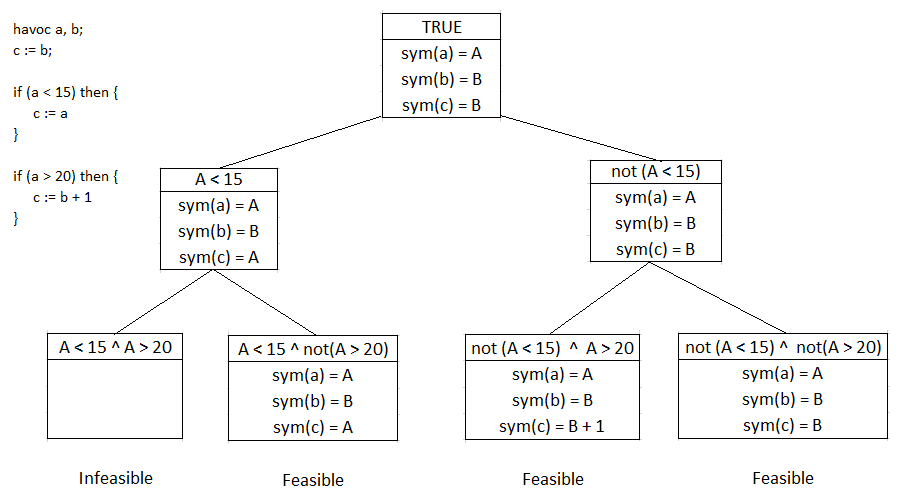
\includegraphics[width=1\textwidth]{SSE_Example.png}
				\caption{Example - Static Symbolic Execution (SSE)} \label{fig_1}
			\end{figure}

		





	\subsection{Dynamic Symbolic Execution (DSE)}
		Dynamic Symbolic Execution is an approach based on concolic execution, which combines both symbolic execution and concrete execution to help guide the engine, when the branch conditions involve operations that are difficult or practically not possible for an SMT solver to check against. Concrete execution essentially drives Symbolic Execution. \cite{2_Survey_SE}.
		
		\vspace{2mm}

		A state in Dynamic Symbolic Execution takes the following form:
		\vspace{-4mm}
		\begin{equation}
			\textbf{$ < $ path-condition, symbolic-environment, concrete-environment $ > $}
		\end{equation}

		Every time a branch condition is reached, one of the branch is executed concretely by checking if the path condition holds for concrete values of variables. This technique was introduced to overcome the problems associated with static symbolic execution with respect to complex operations such as hash algorithms like sha256 which produces outputs that are extremely difficult (next to impossible) to find a satisfying assignment for. It also helped avoid using the solver for 1 branch condition (although it may lead to incompleteness).
		
		\vspace{2mm}

		Today, many different execution engines follow a dynamic approach with different search strategies, with Depth-first search being the most commonly used one.\\

		Following are the search strategies that can or are employed in Dynamic Symbolic Execution:
		\begin{enumerate}
			\item \textbf{Depth-first Style Dynamic Symbolic Execution}
    
				Depth first search (DFS) was one of the first search strategies to be used in Dynamic Symbolic Execution. \cite{1_Search_Strategies_DSE} This strategy makes use of a memory-based model, to track back to the last branch condition. The general steps followed in DFS-based DSE are as follows:\\

				\begin{algorithm}[H]
					\caption{General Steps for Depth-first Style Dynamic Symbolic Execution}  \label{algorithm_2}
					
					\DontPrintSemicolon
					\SetAlgoLined
					
					\KwIn{\textbf{Program AST:}  Abstract Syntax Tree of the program\\
						$\>$ $\>$ $\>$ \textbf{curr\_state:}  Current state in the form of a tuple (path\_condition, symbolic\_environment, concrete\_environment).}
					\KwOut{List of feasible states}
					
					\begin{enumerate}
						\item Get or find concrete environment values.
						\item Concretely keep executing one of the branches, every time a branch condition is reached. Keep doing so, until either – both the branch conditions are infeasible (with concrete values) or until the leaf node has been reached.
						\item Check the last visited branch in memory.
						\item If the other branch condition involves any complex operations, then compute and replace them concretely in the branch condition. Also, concretize all variables involved in performing the complex operations.
						\item Symbolically check if Path-condition (PC) is SATISFIABLE, using an SMT solver.
						\item If PC is SATIFIABLE, then execute the node, else go to step (c).
						\item Repeat from step (b), until no more branches are left to be covered.
					\end{enumerate}
				\end{algorithm}
				~

				It should be noted that the symbolic environment and path condition is always updated with symbolic expressions at each step, irrespective of whether the branch was executed concretely or symbolically. A related example has been covered in \textbf{Section-\ref{Depth-first-style Dynamic Symbolic Execution Engine}} of implementation.
		
				\subsubsection{Benefits}
					\begin{enumerate}
						\item DFS based DSE helps solve the issue associated with complex operations and functions, making constraint solving easier for that branch.
						\item  The number of paths no longer increase in exponential size. Hence, this helps reduce path explosion to some extent.

					\end{enumerate}
					
						
				\subsubsection{Drawbacks}
					\begin{enumerate}
						\item Loses completeness: May not be able to cover all feasible paths.
						\item May get trapped in loops, where the condition does not rely on symbolic inputs. \cite{1_Search_Strategies_DSE}
						\item Size of constraint also increases with growth in execution path, and can potentially make the job of constraint solver harder.
					\end{enumerate}
		
		  %      \vspace{-8mm}
				% \subsubsection{Applications}\hfill\\
				% It is ideal for security applications, which involve a lot of complex cryptographic operations.
               	 		\vspace{-2mm}

				\subsubsection{Examples of real engines in the industry}\
					\begin{enumerate}
						\item DART (Directed Automated Random Testing) \cite{8_DART}
						\item CUTE (Concolic Unit Testing Engine) \cite{9_CUTE}
					\end{enumerate}

				\vspace{8mm}

				
				\item \textbf{Breadth-first Style Dynamic Symbolic Execution} 
				\vspace{1mm}

				Breadth first search (BFS), although not as widely used as DFS, is still utilized by some symbolic execution engines. In BFS, the concrete and symbolic branches are executed in parallel, instead of entirely exploring a particular branch (as in DFS).\cite{1_Search_Strategies_DSE}\\

				The general steps followed in BFS-based Dynamic Symbolic Execution are as follows:\\
				
				\vspace{-3mm}

				\begin{algorithm}[H]
					\caption{General Steps for Breadth-first Style Dynamic Symbolic Execution}  \label{algorithm_3}
					
					\DontPrintSemicolon
					\SetAlgoLined
					
					\KwIn{\textbf{Program AST:}  Abstract Syntax Tree of the program\\
						$\>$ $\>$ $\>$ \textbf{curr\_state:}  Current state in the form of a tuple (path\_condition, symbolic\_environment, concrete\_environment).}
					\KwOut{List of feasible states}
					
					\vspace{2mm}

					\begin{enumerate}
						\item Get or find concrete environment values.
						\item Concretely execute one branch, whichever is feasible with concrete values.
						\item If the other branch condition involves any complex operations, then compute and replace them concretely in the branch condition. Also, concretize all variables involved in performing the complex operations.
						\item In parallel, symbolically execute the other branch.
							\begin{itemize}
								\item Symbolically check if Path-condition (PC) is SATISFIABLE, using an SMT solver.
								\item If PC is SATIFIABLE, then execute the node, else treat the path as infeasible (hence, not explored any further).
							\end{itemize}
						\item Repeat steps (b) to (d) for all the feasible paths in memory – and execute them all in parallel
					\end{enumerate}
				\end{algorithm}
				~

				\textbf{Note:} The symbolic environment and path condition is always updated with symbolic expressions at each step, irrespective of whether the branch was executed concretely or symbolically.

				\vspace{-2mm}

				\subsubsection{Benefits}
					\vspace{1mm}
					\begin{enumerate}
						\item Helps solve the issue associated with complex operation such as cryptographic functions.
						\item Can use the multiprocessor capability of modern systems to traverse each path in parallel.

					\end{enumerate}

				\vspace{-3mm}
					
				\subsubsection{Drawbacks}
					\vspace{1mm}
					\begin{enumerate}
						\item Loses completeness: May not be able to cover all feasible paths.
						\item Memory Utilization is poor:  Since DSE has to keep switching the states. \cite{1_Search_Strategies_DSE}
						\item Exploration space of the program grows quickly. \cite{2_Survey_SE}
					\end{enumerate}

				\vspace{-3mm}

				\subsubsection{Examples of real Engines in Industry}
					\vspace{1mm}
					\begin{enumerate}
						\item EXE \cite{10_EXE}
						\item KLEE \cite{11_KLEE}
					\end{enumerate}
				
				
				\subsubsection{Example}
					.
					\begin{figure}[H]
						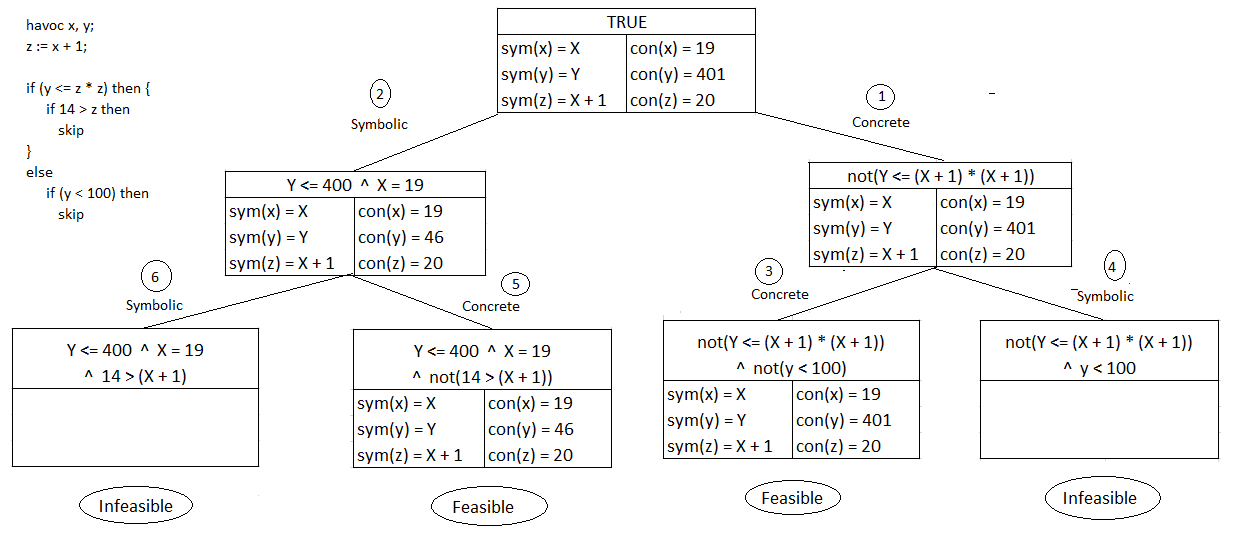
\includegraphics[width=1.17\textwidth]{DSE_BFS_Example.png}
						\caption{Example - Breadth-first Style Dynamic Symbolic Execution} \label{fig_2}
					\end{figure}
		
				\vspace{-12mm}

				% \vspace{-3mm}
		
				% \subsubsection{Applications}\hfill\\
				% Just as DFS style of DSE, it is useful for security applications, which involve a lot of complex cryptographic operations.
				
                \vspace{-3mm}
					
					
			\vspace{9mm}

			\item \textbf{Other Search Strategies:}
	        DFS \& BFS are classical search strategies that do a full traversal of the execution tree of a program but they can be slow for a huge search space.
	        		\vspace{2mm}
			\begin{enumerate}
			    \item \textbf{Random Search:}
			    In this search strategy, execution starts at the root of a program's execution tree and then the execution path is randomly chosen at nodes with conditional statements. This method compromises on stability and does not provide a reliable path coverage but is a quick method to access depth of a program's execution tree in DSE. Hybrid Concolic testing \cite{15_Random} derives from random search but combines it with concolic execution in order to rapidly increase path coverage and thus performing better overall compared to pure DFS or random search.
			   \vspace{3mm}
			    \item \textbf{Heuristic Search Strategies:}
				 Heuristic search strategies aim to solve the issue by trading completeness for speed. They use program context to achieve a fast sub-optimal search space by doing the following: \cite{1_Search_Strategies_DSE}
				\begin{itemize}
					\item Obtain information about the context.
					\item Select the coverage metric.
					\item Compute the weight associated with each feasible path.
				\end{itemize}
                		   \vspace{2mm}
			    Some of the widely used Heuristic Search strategies in dynamic symbolic execution include
				\begin{itemize}
					\item \textbf{Generational Search} which uses ExpandExecution as cost function which is based on path constraints and code coverage criteria.
					\item \textbf{CarFast} which analyses CFG of the program and gives priority to branches containing more states. It is less efficient in DSE when program scale is huge.
					\item \textbf{Control-Flow Directed Search}: starts by creating a CFG of the program and then calculates and assigns weight of each edge. It then selects least weighted path for DSE.
					\item \textbf{Fitness-Guided Search}: solves a fitness function to determine the path to be taken.
					\item \textbf{Context-Guided Search} which, in order to achieve better branch coverage, uses k-context to choose a branch which has a new context for DSE.
				\end{itemize}
			\end{enumerate}
% 			\begin{figure}[H]
% 				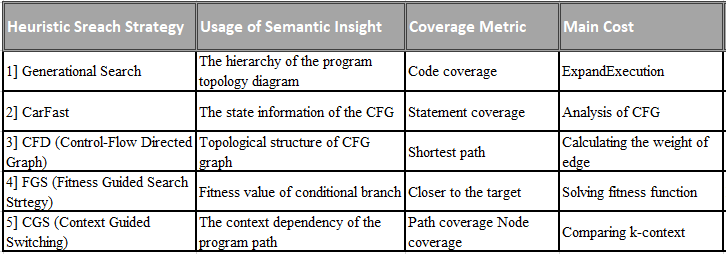
\includegraphics[width=0.95\textwidth]{Heuristic_Search_Strategies_Table.png}
% 				\caption{Heuristic Search Strategies \cite{1_Search_Strategies_DSE}} \label{fig_3}
% 			\end{figure}
		\end{enumerate}

		
	\subsection{Selective Symbolic Execution (SeSE)}
		Sometimes, a developer or team may want to test only a part of the program. In such cases, it’s not useful to run symbolic execution on the entire program. All of the Symbolic execution techniques which we have discussed so far, do not allow for this option. What we want in this case, is a SE engine which takes input from the developer, as to which part of the program he/she intends to perform testing on. \cite{2_Survey_SE} And depending on this input, the engine performs symbolic execution on only the specified part of the program and returns feasible test cases for the respective paths that have been found. The rest of the program can be traversed concretely.\cite{3_SeSE}\\
	
		A state in Selective Symbolic Execution takes the following form:
		\begin{equation}
			\textbf{$ < $ path-condition, symbolic-environment, concrete-environment $ > $}
		\end{equation}

		SeSE creates an illusion of full symbolic execution \cite{3_SeSE}. An important factor to consider here is – “once we encounter and finish performing symbolic execution on the module or part of interest, do we continue symbolically executing the rest of the program, or should we switch back to concrete execution?”


		We will consider both the cases:
		\begin{itemize}
			\item \textbf{The former (Version 1)}  makes sense as the code encountered after the part in contention, would have also been affected by whatever changes were made to that part (perhaps as part of maintenance or update). A proper way to implement this case would be as follows:
				
				\vspace{2mm}

				\begin{algorithm}[H]
					\caption{Selective Symbolic Execution  - General Steps for Version 1}  \label{algorithm_4}
					
					\DontPrintSemicolon
					\SetAlgoLined
					
					\KwIn{\textbf{current\_node:}  Abstract Syntax Tree of the program/block under test\\
						$\>$ $\>$ $\>$ \textbf{curr\_state:}  Current state in the form of a tuple (path\_condition, symbolic\_environment,  concrete\_environment).}
					\KwOut{List of feasible states}\;
		
					\begin{enumerate}
						\item Take concrete input and module/part of interest from the developer/user.
						\item Run SeSE engine concretely till the module\_of\_interest has been encountered.
						\item Once module\_of\_interest is encountered, execute the rest of the program symbolically.
					\end{enumerate}
				\end{algorithm}

			\vspace{2mm}
				
			\item \textbf{The latter (Version 2)} also makes sense in some cases, where the code in contention is meant for specific functionality and has no affect on the rest of the program. A proper way to implement this case would be as follows:

				\vspace{5mm}

				\begin{algorithm}[H]
					\caption{Selective Symbolic Execution  - General Steps for Version 1}  \label{algorithm_5}
					
					\DontPrintSemicolon
					\SetAlgoLined
					
					\KwIn{\textbf{current\_node:}  Abstract Syntax Tree of the program/block under test\\
						$\>$ $\>$ $\>$ \textbf{curr\_state:}  Current state in the form of a tuple (path\_condition, symbolic\_environment,  concrete\_environment).}
					\KwOut{List of feasible states}\;
		
					\begin{enumerate}
						\item Take concrete input and module/part of interest from the developer/user.
						\item Run SeSE engine concretely till the module\_of\_interest has been encountered.
						\item Once module\_of\_interest is encountered, execute the entire module\_of\_interest symbolically.
						\item Once the module\_of\_interest has been fully traversed, execute the rest of the program concretely.
					\end{enumerate}
				\end{algorithm}
		\end{itemize}
		

		\subsubsection{Note:}
			\begin{enumerate}
				\item In the latter case, switching back and forth between symbolic and concrete execution can be a challenging task. We have successfully implemented both the cases with WLANG as the artifact. The results of our implementation have been discussed in detail in \textbf{Section-\ref{Selective Symbolic Execution Engine (SeSE)}} and \textbf{Section-\ref{Comparing and analyzing the 3 implementations with some sample test cases}}.
				\item In Version 1 - the symbolic environment and path condition is always updated with symbolic expressions at each step, irrespective of whether the branch was executed concretely or symbolically. However, in Version 2, we can stop maintaining the symbolic environment, once the module\_of\_interest has been fully traversed.
			\end{enumerate}

		Another major challenge in both the cases is – “how to provide the module/part/code of interest”. There are many different ways to do this. One of the most effective one is to provide the node in AST (Abstract Syntax Tree), corresponding to that module. And this is exactly the approach that we have followed in our implementations of the 2 versions.

		\subsubsection{Examples}
			~\\
			\vspace{1mm}
			- Examples can be found in \textbf{Section-\ref{Selective Symbolic Execution Engine (SeSE)}} and \textbf{Section-\ref{Comparing and analyzing the 3 implementations with some sample test cases}}
		
		\vspace{-1.5mm}

		\subsubsection{Benefits}
			\begin{enumerate}
				\vspace{-0.7mm}
				\item Helps reduce the issues associated with path explosion.
				\item Time associated with constrained solving in now reduced.
			\end{enumerate}
			
		\vspace{-3mm}
			
		\subsubsection{Drawbacks}
			~\\
			\vspace{1mm}
			- Since the part before module\_of\_interest is executed concretely, there is a strong possibility that the module may never be reached. (This can be taken care of, if the developer provides good concrete values instead of using random ones.)

	
	\subsection{Symbolic Backward Execution (SBE)}
		Symbolic Backward Execution, as the name suggests, is a reverse implementation of the traditional Dynamic Symbolic Execution (DSE). It is used to target a specific line of code such as a throw or assert statement in the code which executes in rare cases on very specific input. It helps identify a test suite that can reach that particular line of code and therefore, is an asset for developers while regression testing and debugging.

		\vspace{2mm}
		
		The traversal begins from the leaf node (which is the target) and the constraints of the path condition are collected along the branches in the reverse direction. In SBE, many paths can be traversed at a time. Feasibility is checked periodically, such that unsatisfiable paths are discarded and SBE backtracks. \cite{2_Survey_SE}

		\vspace{2mm}

		\textbf{Requirements of SBE:} Inter-procedural CFG which helps identify call sites for methods in a program should be made available so that the backward traversal is possible \cite{2_Survey_SE}. But even then, it is very difficult to put this into practice.


		\subsubsection{Benefits}
			\begin{enumerate}
				\vspace{-0.7mm}
				\item SBE can help find a test case that can trigger a specific line in the program. 
				\item Multiple paths can be traversed in parallel during SBE. \cite{2_Survey_SE}
				\item Program execution can be traced back from a target line of code to any of the program entry points. \cite{16_sbe}
			\end{enumerate}

		~
		\vspace{1mm}

		As we can see, Symbolic Backward Execution is completely different technique, compared to the ones we've studied so far, in that they go backwards from Leaf nodes.
			
			
		\subsubsection{Drawbacks}
			\begin{enumerate}
				\item Extremely difficult to put into practice since constructing an execution graph with all call sites of a method can be very difficult to construct.
				\item Can be very expensive since a method can have many call sites. \cite{2_Survey_SE}

			\end{enumerate}





\section{Small Implementations of 3 Symbolic Execution Engines in WLANG}
	\subsection{Selective Symbolic Execution Engine (SeSE)}	 \label{Selective Symbolic Execution Engine (SeSE)}
		% {repeating in preset} For implementing this technique, as discussed in the above sections, we are required to provide a reference to the block or code that we wish to execute symbolically. We have used WLANG as our artifact and provide the AST node as the reference to the selected block.\\

		We have implemented 2 versions of the Selective Symbolic Execution techniques:
		\begin{enumerate}
			\item \textbf{Version 1: Concretely executes till the selected block is reached. Symbolically executes the entire code, from the point where the selected block begins}.
				\begin{itemize}
					\item Selective Symbolic Execution can be used to cover only the part that has been changed in the most recent update.
					\item Hence, it is possible that the rest of the execution is also affected due to the changed block. Hence, we symbolically executed the rest of the code, once the selected node or block has been reached.
				\end{itemize}


				~\item \textbf{Version 2: Symbolically executes only the block or node that was selected. Rest of the code, before and after the selected block is executed concretely.}
				\begin{itemize}
					\item We often come across changes or updates in code, which do not have a great deal of effect on the rest of the implementation. Also, sometimes it might be computationally and/or financially very expensive to symbolically execute the code after the selected/updated block.
					\item Hence, in such cases, it is ideal to symbolically execute only the node that has been selected; and leave the rest to be implemented concretely by the CPU (Central Processing Unit) concretely.
				\end{itemize}
		\end{enumerate}

		\subsubsection{Pre-set}
			\begin{itemize}
				\item We are using WLANG as the artifact
				\item Selection of block of code to be tested, is done by reference to ‘AST node’ of the corresponding block.
				\item To simplify the implementation, loop invariants have been supressed.
				\item A state is a tuple (path\_condition, symbolic\_environment, concrete\_environment)\\
					where:
					\begin{itemize}
						\item path\_condition:  List of contraints in symbolic form
						\item symbolic\_environment: A dictionary which maps each defined variable to its symbolic value.
						\item concrete\_environment: A dictionary which maps each defined variable to its concrete value.
					\end{itemize}
			\end{itemize}

		
		\subsubsection{Algorithms (Version 1 v/s Version 2)}
			~\begin{enumerate}
				\item \textbf{Version 1:}
					~

					\begin{algorithm}[H]
						\caption{Selective Symbolic Execution (Version 1)  - \textbf{ version1\_selective\_symbolic\_execution (current\_node, curr\_state, selected\_ast\_node, execution\_type))}}  \label{algorithm_6}
						
						\DontPrintSemicolon
						\SetAlgoLined
						
						\KwIn{\textbf{current\_node:}  Abstract Syntax Tree of the program/block under test\\
							$\>$ $\>$ $\>$ \textbf{curr\_state:}  Current state in the form of a tuple (path\_condition, symbolic\_environment, concrete\_environment). Initially (in the first recursive call) all 3 are empty/NULL.\\
							$\>$ $\>$ $\>$ \textbf{selected\_ast\_node:}  Node to be executed symbolically\\
							$\>$ $\>$ $\>$ \textbf{execution\_type:}  Determines whether the implementation should proceed symbolically or concretely. Initially (in the first recursive call) the value is ‘concrete’.}
						
						\KwOut{List of feasible states}\;
						
						\If {reference (current\_node)  ==  reference (selected\_ast\_node)} {
							execution\_type = ‘symbolic’
						}				
		
						\vspace{2mm}

						list\_feasible\_states = perform\_node\_specific\_execution (current\_node, curr\_state, selected\_ast\_node, execution\_type)
			
						\vspace{2mm}
			
						\If {current\_node.has\_next()} {
						      new\_states = [ ]

							\vspace{1mm}

						       \For{state in list\_ feasible \_states} {
							results = version1\_selective\_symbolic\_execution (current\_node -\> next(), curr\_state, selected\_ast\_node, execution\_type)
			
							\vspace{1mm}
			
							new\_states.extend(results)
						      }\;
						
						      return new\_states
						}
						\Else {
						       return list\_feasible\_states
						}
					\end{algorithm}

					~\\

					Here, the method \textbf{‘perform\_node\_specific\_execution()’} performs the execution (symbolic or concrete – as specified in the argument) and may also involve a call to\textbf{ ‘selective\_symbolic\_execution()’}.

					Note here, that once we find the ‘selected\_node’, the rest of the execution proceeds symbolically.
					\begin{itemize}
						\item The implementation of this algorithm can be found in \textbf{ ‘wlang/SeSE\_v1.py’}.
						\item The examples/tests discussed in this report can be found in \textbf{‘wlang/test\_SSE\_DSE\_SeSE.py’\textbf}.
						\item Some more interesting test cases can be found in \textbf{‘wlang/test\_SeSE\_v1.py’\textbf}.
					\end{itemize}

				\vspace{6mm}


				\item \textbf{Version 2:}
					~

					Here, the method \textbf{‘perform\_node\_specific\_execution()’} performs the execution (symbolic or concrete – as specified in the argument) and may also involve a call to \textbf{‘selective\_symbolic\_execution()’} (for any of the nested nodes - which are a block).  \textbf{‘perform\_node\_specific\_execution()’} also assigns model values to concrete variables (for feasible paths), when branch nodes are reached.\\


					\vspace{3mm}

					\begin{algorithm}[H]
						\caption{Selective Symbolic Execution (Version 2)  - \textbf{ version2\_selective\_symbolic\_execution (current\_node, curr\_state, selected\_ast\_node, execution\_type))}}  \label{algorithm_7}
						
						\DontPrintSemicolon
						\SetAlgoLined
						
						\KwIn{\textbf{current\_node:}  Abstract Syntax Tree of the program/block under test\\
							$\>$ $\>$ $\>$ \textbf{curr\_state:}  Current state in the form of a tuple (path\_condition, symbolic\_environment, concrete\_environment). Initially (in the first recursive call) all 3 are empty/NULL.\\
							$\>$ $\>$ $\>$ \textbf{selected\_ast\_node:}  Node to be executed symbolically\\
							$\>$ $\>$ $\>$ \textbf{execution\_type:}  Determines whether the implementation should proceed symbolically or concretely .Initially (in the first recursive call) the value is ‘concrete’.}
						
						\KwOut{List of feasible states}\;

						flag\_turned = false
						
						\vspace{2mm}

						\If {reference (current\_node)  ==  reference (selected\_ast\_node)} {
							execution\_type = ‘symbolic’\

							\vspace{1mm}

							flag\_turned = true
						}				
		
						\vspace{3mm}

						list\_feasible\_states = perform\_node\_specific\_execution (current\_node, curr\_state, selected\_ast\_node, execution\_type)
			
						\vspace{3mm}

						\If {flag\_turned == true} {
							execution\_type = ‘concrete’
						}

						\vspace{3mm}
			
						\If {current\_node.has\_next()} {
						      new\_states = [ ]
			
							\vspace{1mm}

						       \For{state in list\_ feasible \_states} {
							results = version2\_selective\_symbolic\_execution (current\_node -\> next(), curr\_state, selected\_ast\_node, execution\_type)
							
							\vspace{1mm}
			
							new\_states.extend(results)
						      }\;
						
						      return new\_states
						}
						\Else {
						       return list\_feasible\_states
						}
					\end{algorithm}
					~\\

					\vspace{-3mm}

					Note here, that once we find the ‘selected\_node’, only the ‘node-specific execution’ is performed fully symbolically.

					And the rest of the implementation proceeds concretely.

					\vspace{-1mm}

					\begin{itemize}
						\item The implementation of this algorithm can be found in \textbf{‘wlang/SeSE\_v2.py’}.
						\item The examples/tests discussed in this report can be found in \textbf{‘wlang/test\_SSE\_DSE\_SeSE.py’}.
						\item Some more interesting test cases can be found in \textbf{‘wlang/test\_SeSE\_v2.py’}.
					\end{itemize}
			\end{enumerate}

		\vspace{-3mm}

		\subsubsection{Example}
			~\begin{enumerate}
				\item \textbf{Version 1:} Refer Fig \ref{fig_4}
				\item \textbf{Version 2:} Refer Fig \ref{fig_5}
			~\end{enumerate}

			\textbf{Note that:} in both cases - there is a possibility that the selected node may not be reached.


			\begin{figure}[H]
				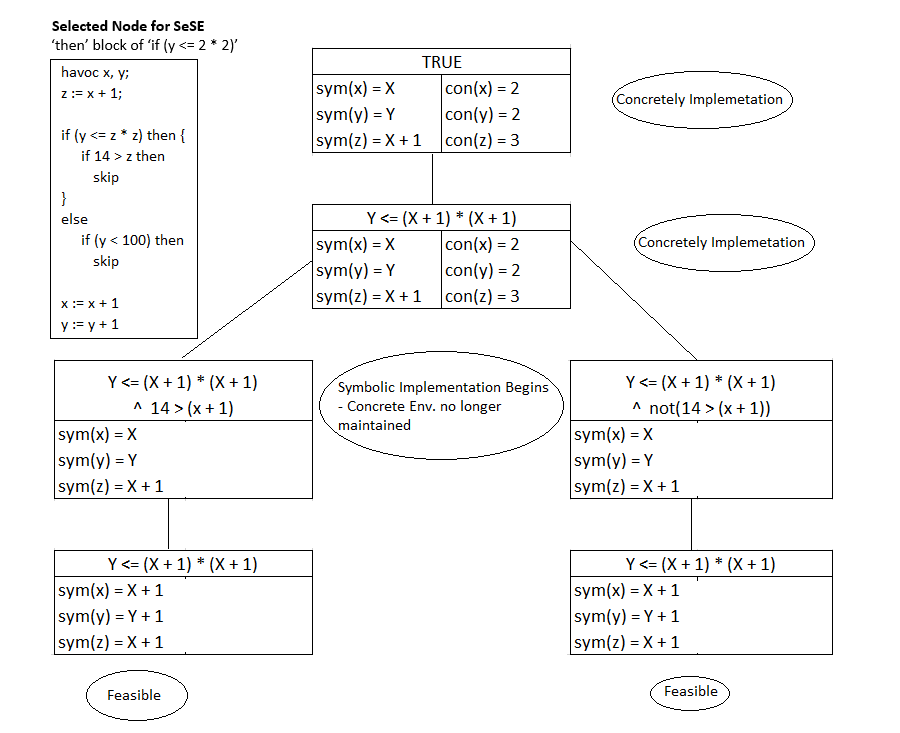
\includegraphics[width=1.05\textwidth]{SeSE_Version1_Example.png}
				\caption{Example - Selective Symbolic Execution (SSE) - Version 1} \label{fig_4}
			\end{figure}
			
			\vspace{-2mm}


	\subsection{Depth-first-style Dynamic Symbolic Execution Engine} \label{Depth-first-style Dynamic Symbolic Execution Engine}
		Here, we are implementing a dynamic approach to symbolic execution in a depth-first manner.
		It is evident that the major benefit of dynamic symbolic execution is the faster processing using CPU for concrete part of the program execution; and in security applications where checking satisfiability of a path condition involving complex operations may be difficult for an SMT solver.

		\vspace{2mm}

		We cover both these aspects in our implementation.
		
		\vspace{2mm}
		
		Since we are using WLANG as the artifact and there is no concept of 'methods' in WLANG, for our implementation, we are considering multiplication (*) and division (/) to be complex operations, which most SMT solvers struggle with.

			\begin{figure}[H]
				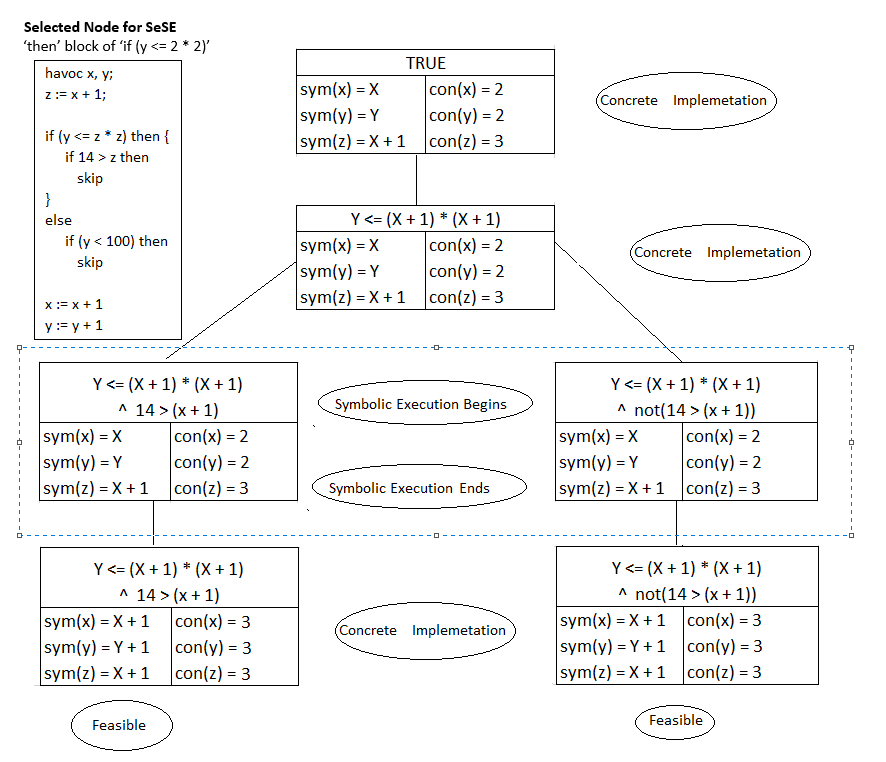
\includegraphics[width=1.05\textwidth]{SeSE_Version2_Example.png}
				\caption{Example - Selective Symbolic Execution (SSE) - Version 2} \label{fig_5}
			\end{figure}

		\vspace{-13mm}

		\subsubsection{Pre-set}
			\begin{itemize}
				\vspace{-2mm}
				\item Using WLANG as the artifact
				\item Complex operations are - multiplication (*) and division (/).
				\item To simplify the implementation, loop invariants have been supressed.
				\item A state is a tuple (path\_condition, symbolic\_environment, concolic\_environment)
				\item Note: For the symbolic branch, we are treating an entire arithmetic expression containing any of the complex operations to be complex expressions, and the symbolic execution proceeds by simplifying the complex expressions using their concrete counterparts.
			\end{itemize}

		\vspace{-5mm}

		\subsubsection{Algorithm}

			\begin{enumerate}
				\vspace{-2mm}
				\item \textbf{find\_concrete\_symbolic():}  Finds the branch that can be satisfied with concrete values and assigns the other branch as symbolic.

				\item \textbf{concretely\_perform\_node\_specific\_execution():}  Concretely executes branch that holds under the concrete values.
					\begin{enumerate}
						\item If any such path exists, then proceeds with that branch-specific execution.
					\end{enumerate}


				\begin{algorithm}[H]
					\caption{Depth-first style Dynamic Symbolic Execution - \textbf{ dynamic\_symbolic\_execution (current\_node, curr\_state)}}  \label{algorithm_8}
					
					\DontPrintSemicolon
					\SetAlgoLined
					
					\KwIn{\textbf{current\_node:}  Abstract Syntax Tree of the program/block under test\\
						$\>$ $\>$ $\>$ \textbf{curr\_state:}  Current state in the form of a tuple (path\_condition, symbolic\_environment, concolic\_environment). Initially (in the first recursive call) all 3 are empty/NULL.}
					
					\KwOut{List of feasible states}\;
					
					branch\_node\_type = [‘if-then-else’, ‘while’, ‘assertion’]
	               
					\vspace{1mm}
	
	              			list\_feasible\_states = [ ]
	
					\vspace{3mm}
					
					\If {‘current\_node.type’  in  ‘branch\_node\_type’} {
						concrete\_branch, symbolic\_branch = find\_concrete\_symbolic (current\_node, curr\_state)
	
						\vspace{1mm}
		
				                     result\_concrete = concretely\_perform\_node\_specific\_execution (concrete\_branch, curr\_state)
	
						\vspace{1mm}
		
				                     result\_symbolic = symbolically\_perform\_node\_specific\_execution (symbolic\_branch, curr\_state)
						
						\vspace{1mm}
				                     
				                     list\_feasible\_states.append (result\_concrete, result\_symbolic)
					}
					\Else {
						 list\_feasible\_states = perform\_node\_specific\_execution (current\_node, curr\_state)
					}
		
					\vspace{3mm}
		
					\If {current\_node.has\_next()} {
						\vspace{1mm}
	
					      new\_states = [ ]
	
						\vspace{1mm}
	
					       \For{state in list\_ feasible \_states} {
						results = dynamic\_symbolic\_execution (current\_node -$>$ next(), curr\_state)
	
						\vspace{1mm}
		
						new\_states.extend(results)
					      }\;
					
					      return new\_states
					}
					\Else {
					       return list\_feasible\_states
					}\;
				\end{algorithm}

				\vspace{2mm}

				\item \textbf{symbolically\_perform\_node\_specific\_execution():}  Symbolically executes the given branch.

					\begin{enumerate}
						\item If:  ‘Path\_Condition’ involves a complex arithmetic expression;

						           - then:  a] Compute the expression concretely and directly replace its value in the ‘path\_condition’

						                         \hspace{10mm} b] Concretize the symbolic variables, which were involved in the complex arithmetic expression.

						           - else: Proceed to ‘Step-(b)’

						\item Check satisfiability.

						\item If:  Satisfiable; then proceed to ‘Step-(d)’

						          - else: Mark as infeasible and  return.

						\item Get the model from SMT solver;  and  assign model values to ‘concrete variables’.
						\item Proceed with the branch specific execution.
					\end{enumerate}
					
				\vspace{0.5mm}
			\end{enumerate}


			\begin{itemize}
				\item  The last 2 methods may also involve a call to ‘selective\_symbolic\_execution()’ (for any of the nested nodes - which are a block)

				\vspace{2mm}

				\item The implementation of this algorithm can be found in \textbf{‘wlang/DSE.py’}.
				\item The examples/tests discussed in this report can be found in \textbf{‘wlang/test\_SSE\_DSE\_SeSE.py’}.
				\item Some more interesting test cases can be found in \textbf{‘wlang/test\_DSE.py’}.
			\end{itemize}

		\subsubsection{Example}
			~\vspace{-4mm}
			\begin{figure}[H]
				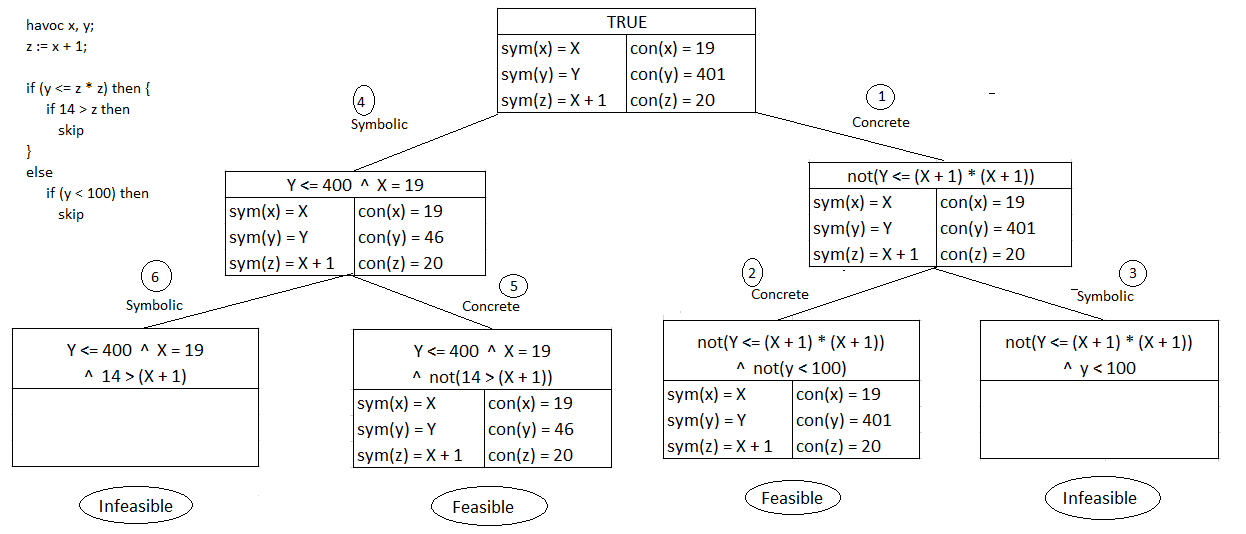
\includegraphics[width=1.05\textwidth] {DSE_DFS_Example.png}
				\caption{Example - Depth First Style Dynamic Symbolic Execution} \label{fig_6}
			\end{figure}



\section{Comparing \& analyzing the 4 implementations with 3 different sample test cases} \label{Comparing and analyzing the 3 implementations with some sample test cases}
	\vspace{-2mm}

	As expected, the time taken by Static Symbolic execution is the maximum of the lot. The freshly implemented techniques (DSE, SeSE-1, SeSE-2) in this project are faster than Static SE which was earlier implemented in Assignment 2. 

	\vspace{2mm}

	But, its also quite abvious that we miss out on completeness with the new techniques. Each of DSE, SeSE-1, and SeSE-2 return a lower number of feasible paths than their static counterpart.

	\vspace{2mm}

	Another very important aspect that we observe here is that each of the 3 new tehniques can potentially return different number of feasible paths, depending on thier initial concrete values. We had randomized our concrete input for the tests, and hence we see the varying results.

	\vspace{2mm}

	Also; time\_taken(SeSE-2) $<$  time\_taken(SeSE-1) $<$  time\_taken(DSE) in most cases; except for example-1, where we get SeSE-1 taking the lowest-time, but that may be due to the small size and structure of the program. The same condition holds for number of paths returned by these techniques; i.e.: \#paths(SeSE-2) $<$  \#paths(SeSE-1) $<$ \#paths(DSE)
	
   	 \vspace{2mm}

	It maybe noted that for DSE, if we run the test cases, and print the feasible states; then we will observe that concrete branch also has a simplified value for the complex sub-expressions. This is essentially because, any symbolic path further down this branch may again need to be concretized to solve for these complex expressions and that too with the same concrete value that the symbolic path at previous branch was simplififed with (if any). Hence, instead of repeating this procedure, it makes sense to simplify the path for the concrete branch where it first observed that complex expression. This will hold for the concrete split going further and for symbolic split, since we would have had to essentially repeat the same procedure with the same concrete values again, this would also hold for it.
	
	\vspace{-4mm}

	\begin{figure}[H]
		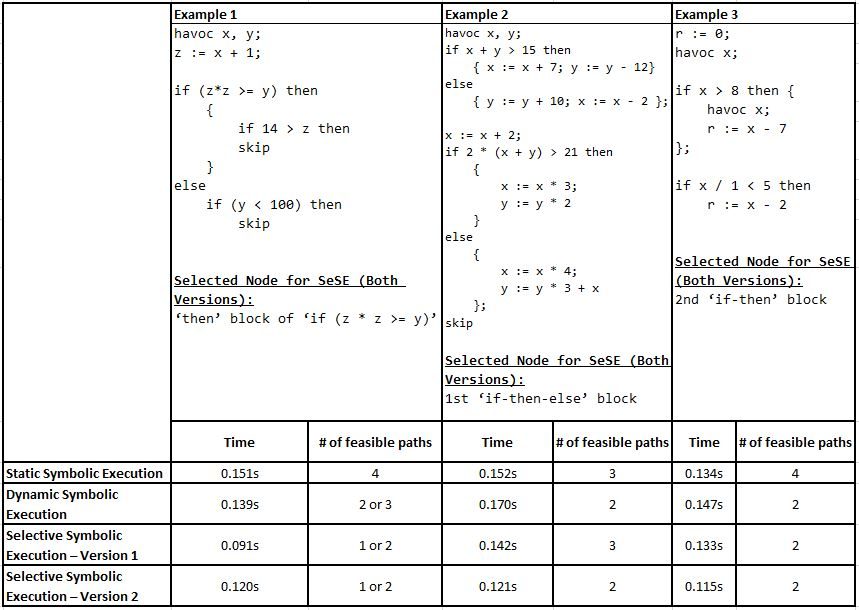
\includegraphics[width=1.1\textwidth]{Analysis.JPG}
		\caption{Analyzing the 4 implementations with some sample test cases} \label{fig_7}
	\end{figure}

	\vspace{-5mm}

\section{Conclusion}
	As we observed through our analysis, we can adopt different techniques of symbolic execution and also in different configurations to tackle the problems associated with Static or Classical symbolic execution, most particular being 'path explosion' and 'complex operations'.

	\vspace{2mm}

	The symbolic execution techniques have been listed in \textbf{Fig-\ref{fig_7}} in decreasing order of their association with symbolic activity. And hence we observe a lower time, required for symbolic processing, while the no. of feasible paths also decrease; from SSE to DSE to SeSE-1 to SeSE-2.

	\vspace{2mm}

	While SeSE may be the fastest techniques of the lot, they are not always practical in real-life. DSE is the most widely used technique, as it helps reduce path explosion and saves computing resources utilized by the solver; while also maintaining a relatively higher level of symbolic association.

	\vspace{2mm}

	Depending on the case and context, a developer or organization may choose to utilize any of these techniques or may even try and come up with thier own version of symbolic execution.	

	\vspace{5mm}
%
% ---- Bibliography ----
%
% BibTeX users should specify bibliography style 'splncs04'.
% References will then be sorted and formatted in the correct style.
%
% \bibliographystyle{splncs04}
% \bibliography{mybibliography}
%
\begin{thebibliography}{9}
\bibitem{1_Search_Strategies_DSE}
Yu LIU*, Xu ZHOUa and Wei-Wei GONGb.:  A Survey of Search Strategies in the Dynamic Symbolic Execution \url{https://www.itm-conferences.org/articles/itmconf/abs/2017/04/itmconf_ita2017_03025/itmconf_ita2017_03025.html}

\bibitem{2_Survey_SE}
ROBERTO BALDONI, EMILIO COPPA, DANIELE CONO D’ELIA, CAMIL DEMETRESCU, and IRENE FINOCCHI, Sapienza University of Rome.:  A Survey of Symbolic Execution Techniques \url{https://arxiv.org/abs/1610.00502}

\bibitem{3_SeSE}
Vitaly Chipounov, Vlad Georgescu, Cristian Zamfir, George Candea School of Computer and Communication Sciences ´E cole Polytechnique F´ed´erale de Lausanne (EPFL), Switzerland.:  Selective Symbolic Execution \url{https://infoscience.epfl.ch/record/139393}

\bibitem{4_TP_SE}
Tutorials Point, Software testing dictionary, \url {https://www.tutorialspoint.com/software_testing_dictionary/symbolic_execution.htm}


\bibitem{5_Wiki_SE}
Wikipedia, Symbolic Execution, \url {https://en.wikipedia.org/wiki/Symbolic_execution}


\bibitem{6_MS_Z3}
Micrisoft Research, z3,  \url {https://www.microsoft.com/en-us/research/project/z3-3/}

\bibitem{7_UW_SE}
University of Waterloo, ECE 653, Symbolic Execution,  \url {https://git.uwaterloo.ca/stqam-1225/pdfs/-/raw/master/W05-SymExec.pdf}

\bibitem{8_DART}
 Patrice Godefroid Nils Klarlund, Koushik Sen.:  DART: Directed Automated Random Testing,  \url {https://web.eecs.umich.edu/~weimerw/590/reading/p213-godefroid.pdf}

\bibitem{9_CUTE}
 Koushik Sen, Darko Marinov, Gul Agha.:  CUTE: A Concolic Unit Testing Engine for C  \url {https://mir.cs.illinois.edu/marinov/publications/SenETAL05CUTE.pdf}

\bibitem{10_EXE}
Cristian Cadar, Vijay Ganesh, Peter M. Pawlowski, David L. Dill, Dawson R. Engler.:  EXE: Automatically Generating Inputs of Death,  \url {https://dl.acm.org/doi/10.1145/1455518.1455522}

\bibitem{11_KLEE}
KLEE, Github IO,  \url {11.	https://klee.github.io/}

\bibitem{12_UW_DSE}
University of Waterloo, ECE 653, Dynamic Symbolic Execution,  \url {https://git.uwaterloo.ca/stqam-1225/pdfs/-/raw/master/W06-DSE.pdf}

\bibitem{13_MS_SAGE}
Patrice Godefroid, Michael Y. Levin, David Molnar, Microsoft.:  SAGE: Whitebox Fuzzing for Security Testing ,  \url {https://queue.acm.org/detail.cfm?id=2094081}

\bibitem{14_DirSE}
Kin-Keung Ma, Khoo Yit Phang, Jeffrey S. Foster, and Michael Hicks:  Directed symbolic execution,  \url {https://www.cs.umd.edu/~mwh/papers/dse-sas11.pdf}

\bibitem{15_Random}
Majumdar, Rupak, and Koushik Sen. "Hybrid concolic testing." 29th International Conference on Software Engineering (ICSE'07). IEEE, 2007.

\bibitem{16_sbe}
Peter Dinges and Gul Agha. 2014. Targeted test input generation using symbolic-concrete backward execution. In Proceedings of the 29th ACM/IEEE International Conference on Automated Software Engineering (ASE’14). 31–36. DOI,  \url{http://dx.doi.org/10.1145/2642937.2642951}

\end{thebibliography}
\end{document}
